
\documentclass{article}
%%%%%%%%%%%%%%%%%%%%%%%%%%%%%%%%%%%%%%%%%%%%%%%%%%%%%%%%%%%%%%%
%%                    ** mymacros.tex **                     %%
%%%%%%%%%%%%%%%%%%%%%%%%%%%%%%%%%%%%%%%%%%%%%%%%%%%%%%%%%%%%%%%


\typeout{** loading mymacros.tex **}

\def\h{\hbox}

\newcommand{\mathcom}[3]{ \newcommand{#1}[#2]{\mbox{$#3$}}}
\newcommand{\remathcom}[3]{ \renewcommand{#1}[#2]{\mbox{$#3$}}}

\newcommand{\mdef}[2]{ \newcommand{#1}{\mbox{$#2$}} }
 
\mathcom{\y}{0}{\ \vdash\ }               % yeilds 
\mathcom{\ys}{0}{\vdash_{\cal S}}         % yeilds sub S
\mathcom{\yt}{0}{\vdash_{\theta}}         % yeilds sub theta

\mathcom{\absurd}{0}{\mathbf{f}}                 % absurdity
\mathcom{\imp}{0}{\ \rightarrow\ }            % implication arrow
\mathcom{\rimp}{0}{\ \leftarrow\ }            % implication arrow

\mathcom{\con}{0}{\ \wedge\ }                 % conjunction
\mathcom{\dis}{0}{\ \vee\ }                   % disjunction
\mathcom{\n}{0}{\neg}                     % negation
\mathcom{\dimp}{0}{\ \leftrightarrow\ }       % mat equiv

\mathcom{\corresponds}{0}{\ \Lleftarrow\! \! \Rrightarrow\ }


%%\mathcom{\th}{0}{\theta}                  % theta


\mathcom{\A}{0}{\forall}                  % universal quantifier
\mathcom{\E}{0}{\exists}                  % existential quant

\mathcom{\Dec}{1}{{\cal D}(#1)}           % D(#1)

\mathcom{\elt}{0}{\in}

\mathcom{\tuple}{1}{\langle #1 \rangle}

% \mathcom{\equivdef}{0}{\equiv_{\mbox{\em \tiny def}}}
% \mathcom{\eqdef}{0}{=_{\mbox{\em \tiny def}}}
\def\equivdef{\mathrel{\ \equiv_{\mbox{\em \tiny
def}}\ }}

\def\eqdef{\mathrel{\ =_{\mbox{\em \tiny def}}\ }}


% \newtheorem{Rule}{Rule}
% \newtheorem{Lemma}{Lemma}
% \newtheorem{Theorem}{Theorem}


% Redeclaration of symbols for intuitionistic logic
% see Diller p.126
\def\ineg{\mathop\sim}
\def\iimp{\mathbin\Rightarrow}
\def\iiff{\mathbin\Leftrightarrow}
% new symbols from amssymb
%\def\iimp{\mathbin\rightarrowtail}
%\def\iiff{\mathbin\leftrightsquigarrow}

\def\icon{\mathbin\curlywedge}
\def\idis{\mathbin\curlyvee}

%Definitions for RCC inserts
\newcommand{\notch}{\Longrightarrow\kern-16pt{/}\ \ \ }
\newcommand{\ch}{\Longrightarrow}
\newcommand{\pr}[1]{\mbox{\sf #1}}

% RCC relations
\mathcom{\C}{0}{\pr{C}}
\remathcom{\P}{0}{\pr{P}}
\remathcom{\O}{0}{\pr{O}}
\mathcom{\PO}{0}{\pr{PO}}
\mathcom{\PP}{0}{\pr{PP}}
\mathcom{\NTPP}{0}{\pr{NTPP}}
\mathcom{\NTPPI}{0}{\pr{NTPP}^{-1}}
\mathcom{\TPP}{0}{\pr{TPP}}
\mathcom{\TPPI}{0}{\pr{TPP}^{-1}}
\mathcom{\TP}{0}{\pr{TP}}
\mathcom{\NTP}{0}{\pr{NTP}}
\mathcom{\NTPi}{0}{\pr{NTPi}}
\mathcom{\EC}{0}{\pr{EC}}
\mathcom{\DC}{0}{\pr{DC}}
\mathcom{\DR}{0}{\pr{DR}}
\mathcom{\EQ}{0}{\pr{EQ}}
\mathcom{\CG}{0}{\pr{CG}}

\mathcom{\Pin}{0}{\pr{Pi}} % \Pi is Greek letter
\mathcom{\PPi}{0}{\pr{PPi}}
\mathcom{\NTPPi}{0}{\pr{NTPPi}}

\mathcom{\OP}{0}{\pr{OP}}

\mathcom{\conv}{0}{\pr{conv}}
\mathcom{\rsum}{0}{\pr{sum}}
\mathcom{\rdiff}{0}{\pr{diff}}
\mathcom{\rcompl}{0}{\pr{compl}}
\mathcom{\rprod}{0}{\pr{prod}}
\mathcom{\cp}{0}{\pr{cp}}
\mathcom{\Us}{0}{\pr{Us}}
\mathcom{\us}{0}{\pr{u}}
\mathcom{\NULL}{0}{\pr{NULL}}
\mathcom{\rnull}{0}{\emptyset}
\mathcom{\CONV}{0}{\pr{CONV}}
\mathcom{\CON}{0}{\pr{CON}}

% Adaptations for new latex compatibility
\renewcommand{\Box}{\square}
\def\cal{\mathcal}

% meta language in definitions etc
\mathcom{\ml}{1}{\;\;\;\; \mbox{#1} \;\;\;\;}


%-- TOPLOG SYMBOLS

\mathcom{\Co}{0}{{\cal C}_{0} \ }
\mathcom{\CoX}{0}{{\cal C}_{0}}
\mathcom{\Cop}{0}{{\cal C}_{0}^+ \ }
\mathcom{\CopX}{0}{{\cal C}_{0}^+}
\mathcom{\mcop}{0}{\models_{C_o^+}}

\mathcom{\Lop}{0}{{\cal L}_{0}^+ \ }
\mathcom{\LopX}{0}{{\cal L}_{0}^+}
\def\mlo{\models_{{\mathcal  L}_0}}
\def\mlop{\models_{{\mathcal  L}_0^+}}

\mathcom{\Ci}{0}{{\cal C}_{1} \ }
\mathcom{\CiX}{0}{{\cal C}_{1}}

\mathcom{\Io}{0}{{\cal I}_{0} \ }
\mathcom{\IoX}{0}{{\cal I}_{0}}
\mathcom{\Iop}{0}{{\cal I}_{0}^+ \ }
\mathcom{\IopX}{0}{{\cal I}_{0}^+}

%%\mathcom{\inter}{1}{\langle #1 \rangle}
\mathcom{\inter}{1}{i( #1 )}

\newfont{\myssfont}{cmss12}

\mathcom{\Maps}{2}{\, _{#1}\!\!\!\rightleftharpoons^{#2} \ }

\mathcom{\CotoST}{0}{\Maps{C_0}{ST}}
\mathcom{\CtoST}{0}{\Maps{C\,}{ST}}
\mathcom{\IotoST}{0}{\Maps{I_0}{ST}}

\mathcom{\uni}{0}{\cal U \, }
\mathcom{\uniX}{0}{\cal U}
\mathcom{\U}{0}{\cal U}

\mathcom{\eu}{0}{\,=\,\uni}

\mathcom{\ol}{1}{\overline{#1}}

\mathcom{\Lsse}{0}{{\cal L}_{sse}}
\mathcom{\Lssei}{0}{{\cal L}_{ssei}}

\mathcom{\Luse}{0}{{\cal L}_{use}}
\mathcom{\Lusei}{0}{{\cal L}_{usei}}

\mathcom{\disdots}{0}{\dis\!\!\!\ldots\!\!\dis}
\mathcom{\condots}{0}{\con\ldots\con}





%% Miscelleneous


\def\HA#1#2{\pr{Holds-At}(#1,#2)}
\def\col{\!:\!}

% Enclose arguments in square double brackets to
% refer to semantic value of an expression
\def\semvalue#1{[\mkern-3mu[#1]\mkern-3mu]}

\def\forces{\mathop{\setbox0=\hbox{$\vdash$}\ \rule{0.04em}{1\ht0}\mkern1.5mu\box0}}

\mathcom{\hence}{0}{\Longrightarrow \hspace{2em}}

\def\sliderule{\centerline{\rule{4in}{1mm}}}

\def\Cbox{\mathop{\square\mkern-10mu
                   \mbox{\raise0.45ex\hbox{\tiny\sf C}}
                  \mkern2mu
                 }
         }

\def\letterbox#1{\mathop{\square\mkern-10mu
                   \mbox{\raise0.2ex\hbox{\small\sf #1}}
                  \mkern2mu
                 }
         }

%\def\tBox{\letterbox{\lower0.4ex\hbox{t}}}
\def\sBox{\letterbox{s}}
\def\tBox{\letterbox{t}}

\def\overstrike#1#2{\mathop{%
               \setbox1=\hbox{$#1$}%
               \setbox2=\hbox{$#2$}%
               \ifdim 1\wd1<1\wd2 % 
                    { \rlap{\mbox{\kern0.5\wd2\kern-0.5\wd1 \box1}} \box2 }
              \else {   \rlap{\mbox{$#1$}}
                        \rlap{\mbox{\kern0.5\wd1\kern-0.5\wd2 \box2}}
                        \phantom{#1} } 
              \fi }}

\def\rbox{\boxminus}
\def\rdia{\overstrike{\Diamond}{-}}
\def\cdia{\overstrike{\Diamond}{\rule{0.04em}{1.5ex}}}
\def\cbox{\inbox{\rule{0.04em}{1.6ex}}}
\def\cbox{\mathop{\setbox0=\hbox{$\square$}
                  \overstrike{\square}{\hbox{\rule{0.04em}{1\ht0}}}
             }}

\def\diaplus{\overstrike{\Diamond}{+}}




%% Make a modal box with a symbol centred inside
\def\inbox#1{\mathop{\setbox0=\hbox{$\square$}%
                      \setbox1=\hbox{#1}%
                      \rlap{\hbox{$\square$}}
                      \rlap{\mbox{\kern0.5\wd0\kern-0.5\wd1%
                                  \box1}}%
                      \phantom{\square}}}

\def\ibox{\mathop{\square\mkern-10mu
                   \mbox{\raise0.45ex\hbox{\tiny\em i}}
                  \mkern7mu
                 }
         }
\def\cdiamond{\mathop{\Diamond\mkern-12.7mu
                   \mbox{\raise0.4ex\hbox{\tiny\em c}}
                  \mkern7mu
                 }
         }


\def\s5box{\mathop{\square\mkern-10mu
                   \mbox{\raise0.45ex\hbox{\tiny 5}}
                  \mkern7mu
                 }
         }

\def\Fbox{\mathop{\square\mkern-11mu
                   \mbox{\raise0.45ex\hbox{\tiny \bf F}}
                  \mkern2mu
                 }
         }

\def\Box{\mathop\square}
\def\Diamond{\mathop\lozenge}

\def\bigI{\mathop{%
\hbox{%
%%
\def\thickness{1pt}%
\def\width{6pt}%
\def\height{0.6em}%
\def\gap{0.15em}%
%%
\dimen0=\thickness%
\divide\dimen0 by 2%
\dimen1=\width%
\divide\dimen1 by 2%
%%
\kern\gap%
\rlap{\vrule width\width height\thickness depth0pt}%
\rlap{\kern\dimen1 \kern-\dimen0%
\vrule width\thickness height\height depth0pt}%
\raise\height\hbox{\vrule width\width height\thickness depth0pt}%
\kern\gap}}}

\def\mconv{\mathop{% 
      \mbox{\raise0.35ex\hbox{$\scriptstyle\bigcirc$}}
                  }
          }
\def\mpconv{\circleddash}



% \def\putat#1#2#3{\setbox1=\hbox{#3}%
% \rule{0pt}{0pt}%
% \vspace*{#2}%
% \hspace*{#1}%
% \rule{0pt}{0pt}%
% \hbox to 0em{\rlap{\vtop to 0ex{\hbox to 0em{#3}}}}%
% \hspace*{-#1}\vspace*{-#2}}
% %\rule{0pt}{0pt}
% %\vspace*{-\ht1}\rule{0pt}{0pt}
% %\vspace*{-\ht1}

\def\putat#1#2#3{\rlap{\hbox{%
\kern#1% 
\vtop{\hbox{}%
\hbox{\vbox to #2{}} \hbox{#3}}}}}

% use putat within \hbox
% Objects will be located relative to baseline
% at start of the \hbox
% eg:
% \hbox{
% \putat{2in}{2in}{xxxxx}%
% \putat{2in}{2in}{00000}%
% \putat{5in}{3in}{Z}%
% \putat{2in}{2in}{0}%
% \putat{5in}{4in}{x}%
% }


%\long\def\putat#1#2#3{




\def\ri{\mathclose{\raise1ex\hbox{$\smile$}}}

\def\eqtag#1{\eqno ({\bf #1})}

\def\mc:#1{\hbox{${\mathcal{#1}}$}}
\def\mb#1{{\mathbf{#1}}}
 
\def\ifff{\qquad \hbox{if and only if} \qquad}

%%\def\d{\delta}

\def\QED{$\blacksquare$}

\def\epsrcgrant{GR/K65041}
\def\VUGgrant{GR/M56807}

\def\Boxx{\boxtimes}

%% Force a math symbol to go into scriptsize
\def\mscriptsize#1{\hbox{\scriptsize $#1$}}
\def\mlarge#1{\hbox{\large $#1$}}

\def\boxtheorem#1#2{~\\
\centerline{\fbox{
\parbox{5in}{
\centerline{\bf #1}
#2
}}}
\vspace{1ex}}

\def\proof#1#2{
\begin{quotation}
\noindent {\bf Proof of #1:}
#2
\QED
\end{quotation}
}

\def\proofpar{\\ \hspace*{1.5em}}


%%%% ENVIRONMENTS

%% specify my list parameters
%% These can be overridden by declarations within
%% a document.

\def\mytopsep{1ex}
\def\mypartopsep{0ex}
\def\myitemsep{0.3ex}
\def\myparsep{0ex}
\def\mylistparindent{2em}
\def\myleftmargin{4.5em}
\def\mylabelwidth{4.5em}
\def\mylabelsep{1em}
\def\myitemindent{0em}

\def\setmylistparams{%
             \setlength{\topsep}{\mytopsep}
             \setlength{\partopsep}{\mypartopsep}
             \setlength{\itemsep}{\myitemsep}
             \setlength{\parsep}{\myparsep}
             \setlength{\listparindent}{\mylistparindent}
             \setlength{\leftmargin}{\myleftmargin}
             \setlength{\labelwidth}{\mylabelwidth}
             \setlength{\labelsep}{\mylabelsep}
             \setlength{\itemindent}{\myitemindent}
        }

\def\clistbullet{$\bullet$}

\newcounter{tempvalue}
% A compact list making environment
\newenvironment{clist}
    { %\vspace{1ex}
      \begin{list}
            {\labelitemi}
            \setmylistparams
    }
    { \end{list}\addvspace{1ex} 
    }
% A compact list making environment
% with -- as the default item tag
\newenvironment{cdashlist}
    { %\vspace{1ex}
      \begin{list}
            {--}
            {\setlength{\topsep}{0.2ex}
             \setlength{\partopsep}{0ex}
             \setlength{\itemsep}{0.3ex}
             \setlength{\parsep}{0ex}
             \setlength{\listparindent}{2em}
            }
    }
    { \end{list}\addvspace{1ex} 
    }


% compact list with wide labels for item tags
\newenvironment{taglist}[1]
    { %\vspace{1ex}
      \begin{list}
            {$\bullet$}
            {\setlength{\topsep}{0.2ex}
             \setlength{\partopsep}{0ex}
             \setlength{\itemsep}{0.3ex}
             \setlength{\parsep}{0ex}
             \setlength{\listparindent}{2em}
             \setlength{\leftmargin}{#1}
             \setlength{\labelwidth}{#1}
             %\addtolength{\labelwidth}{-1em}
             \setlength{\labelsep}{0em}
            }
    }
    { \end{list}\addvspace{1ex} 
    }

\newcounter{cenumcount}
\newenvironment{cenum}
    { %\vspace{1ex}
      \begin{list}
            {\arabic{cenumcount}.}
            {\usecounter{cenumcount}
               \setmylistparams
            }
    }
    { \end{list}\addvspace{1ex} 
    }

\newcounter{romcount}
\newenvironment{romanenum}
          { 
            \begin{list}{\roman{romcount})~~}
                        {\usecounter{romcount}
                         \setmylistparams
                        }
          }
          { \end{list} }

\newcounter{alphcount}
\newenvironment{alphenum}
          { \begin{list}{\alph{alphcount})~~}
                        {\usecounter{alphcount}}}
          { \end{list} }


%% Labelled list environment
\newenvironment{llist}[1]{%
\newcounter{#1}
\begin{list}{({\bf #1\arabic{#1}})\hspace{1em}}{\usecounter{#1}}
}
{\end{list}}

%% Labelled list continued
%% (assumes counter already exists)
\newenvironment{llistcont}[1]{%
\setcounter{tempvalue}{\value{#1}}
\begin{list}{({\bf #1\arabic{#1}})\hspace{1em}}{%
\usecounter{#1}
\setcounter{#1}{\value{tempvalue}}
}
}
{\end{list}}

%%% compact versions of llist and llistcont
\newenvironment{cllist}[1]{%
\newcounter{#1}
\begin{list}{({\bf #1\arabic{#1}})}
             { \usecounter{#1}
               \setmylistparams
             }
}
{\end{list}}

%% Labelled list continued
%% (assumes counter already exists)
\newenvironment{cllistcont}[1]{%
\setcounter{tempvalue}{\value{#1}}
\begin{list}{({\bf #1\arabic{#1}})}{%
                 \usecounter{#1}
                 \setcounter{#1}{\value{tempvalue}}
                \setmylistparams
          }
}
{\end{list}}


\def\longdef{\long\def}

%% Define a labelled list type
%% #1 name of control sequence for the list type
%% #2 prefix for numbering
\def\llisttype#1#2{%
\newcounter{#2}
\expandafter\longdef\csname #1list\endcsname##1{%
\begin{cllistcont}{#2}
##1
\end{cllistcont}}
\expandafter\def\csname #1\endcsname##1{%
\begin{cllistcont}{#2}
\item
##1
\end{cllistcont}}
}

\def\litem#1#2{%
\begin{clist}
\item[({\bf #1})] 
#2
\end{clist}}

\newenvironment{chapabst}%
{\begin{quotation}\small\noindent }{\end{quotation}}

% Split line displayed formulae
% (not actually an environment)
\newcommand{\splitdismath}[4]{%
{\setlength{\arraycolsep}{0em}
\begin{eqnarray}
& #1 & #2 \nonumber \\
 &    & #3 
\label{#4}
\end{eqnarray}
}
}

% Displayed equation with tabbing

\newcommand{\tabmathn}[2]
{ \begin{equation}
\vbox{
\vspace{-2ex}
\begin{tabbing}
#1
\end{tabbing}
\vspace{-3.5ex}
}
\label{#2}
\end{equation}
}

\newcommand{\displaytab}[1]
{ \begin{displaymath}
\vbox{
\vspace{-2ex}
\begin{tabbing}
#1
\end{tabbing}
\vspace{-3.5ex}
}
\end{displaymath}
}

\def\myeq#1{$$\eqalign{#1}$$}


%%% Reinstate \eqalign macros removed by Lamport
\catcode`\@=11
\def\eqalign#1{\null \,\vcenter {\openup \jot \m@th 
\ialign {\strut \hfil $\displaystyle{##}$&$\displaystyle {{}##}$\hfil
 \crcr #1\crcr }}\,}

\def\eqalignno#1{\displ@y \tabskip \centering 
\halign to\displaywidth {\hfil $\@lign \displaystyle{##}$\tabskip \z@skip
 &$\@lign \displaystyle {{}##}$\hfil \tabskip \centering 
 &\llap {$\@lign ##$}\tabskip \z@skip \crcr 
 #1\crcr }}

\def\leqalignno#1{\displ@y \tabskip \centering
 \halign to\displaywidth {\hfil $\@lign \displaystyle {##}$\tabskip \z@skip
 &$\@lign \displaystyle {{}##}$\hfil \tabskip \centering
 &\kern -\displaywidth \rlap {$\@lign ##$}\tabskip \displaywidth \crcr 
 #1\crcr}}

%%% Define something like \bibliography but only records the
%%% bibfiles (does not input the bbl file)
\def\bibliographyfiles#1{%
  \if@filesw
    \immediate\write\@auxout{\string\bibdata{#1}}%
  \fi}

%%% Define a separate command to input the bbl file.
\def\bibliographytext{%
  \@input@{\jobname.bbl}}


%% Suppress printing of bibitems in thebibliography
%% This is for use with the `inlinebib' package,
%% which adds fullcitations where you give the \cite command.
%% Doesn't print note
%% Could add note by changing ##2 to ##2##3 in the \bibcite argument
%% But output not quite right.
\def\suppressendbib{%
\long\def\@bibitem##1 ##2 \note ##3 \short ##4 \end{\par\if@filesw
        {\def\protect####1{\string ####1\space}%
         \let\newblock\@empty
         \immediate\write\@auxout{\string
                \bibcite{##1}{\string\@bibcall{##1}{##2}{##4}}}}\fi
        }
\def\thebibliography##1{}
}


%% Change indent space allocated by \thebibliography
%% use before \bibliography or \bibliographytext 
\def\setbibindent#1{%
\let\oldthebibliography\thebibliography
\def\thebibliography##1{\oldthebibliography{#1}}
}



\catcode`\@=12

\long\def\skipover#1{}

\long\def\correction#1{\footnote{TO CORRECT: #1}}
\def\nocorrections{\long\def\correction##1{}}
\def\question#1{{\bf Question:} {\em #1} }
\long\def\todo#1{{\bf To Do:} {\em #1} }


\def\twiddle{$\sim$}

%% Macro for URLs
%% puts them in tt format and  breaks line after dot if needed.

\skipover{
\def\urlspace{-0.5em}
\def\url#1{{\tt \urlsub#1\end}}
%\def\urldot{. \hspace{-1em}\urlsub}
\def\urldot{. \linebreak[1]\hspace\urlspace\urlsub}
\def\urlcolon{: \linebreak[1]\hspace\urlspace\hspace\urlspace\urlsub}
\def\urlslash{/ \linebreak[1]\hspace\urlspace\urlsub}
\def\urltilde{\twiddle\urlsub}
\def\urlsub#1{\ifx#1\end \let\next=\relax
      \else \ifx#1.\let\next=\urldot
      \else \ifx#1:\let\next=\urlcolon
      \else \ifx#1/\let\next=\urlslash
      \else \ifx#1~\let\next=\urltilde
      \else#1\let\next=\urlsub\fi\fi\fi\fi\fi\next}
}

% Input a file in verbatim mode (eg a program file)
\def\verbinput#1{\expandafter\begin{verbatim}\input#1}
%NB: usage: \verbinput{filename}\end{verbatim}


\def\mb#1{{\mathbf{#1}}}
\def\mbf#1{{\mathbf{#1}}}


%%% MACROS for SLIDES


\def\heading#1{%
\centerline{\shadowbox{
\large \begin{tabular}{c} #1 \end{tabular}
           }  }
\vspace{1ex minus 1ex}
}

\def\bheading#1{%
\centerline{\shadowbox{
\large\bf \begin{tabular}{c} #1 \end{tabular}
           }  }
\vspace{1ex minus 1ex}
}

\def\printlandscape{\special{landscape}}    % Works with dvips.
\def\printportrait{\special{portrait}}

\def\leedslogo#1{\centerline{
\psfig{file=uol.eps,width=#1} %% May look wrong in xdvi
}}

\def\titleslide#1#2{
\begin{slide*}
~

\vfill
\heading{#1}

\vfill
\begin{center}
        {\large\bf Brandon Bennett} 

\vspace{3ex}
        Division of AI \\
        School of Computing \\
        University of Leeds\\ 
        Leeds LS2 9JT, England \\
        {\tt brandon@comp.leeds.ac.uk} \\
\end{center}

\vfill
\centerline{
\psfig{file=uol.eps,width=0.7in} %% May look wrong in xdvi
}
\vfill
\centerline{#2}
\vfill
\end{slide*}
}


\def\nlf{\\ \mbox{} \hfill}

%%\def\fixhyphens{\usepackage[english]{babel}}

%% FIX HYPHENATION
\lefthyphenmin=2
\righthyphenmin=3

%% special commands for spell checker
\def\sic#1{#1}
\def\sico!#1!{#1}
\def\sicname#1{#1}
\def\accept#1{}
\def\acceptname#1{}

%\newenvironment{nospell}{}{}
\def\spelloff{}
\def\spellon{}


%% Check whether a macro is defined
\def\ifundefined#1{\expandafter\ifx\csname#1\endcsname\relax}

%% Define \ifpdf
%% Used in graphic stuff to check if pdf is running
%% This is taken from ifpdf.sty
\newif\ifpdf
\ifx\pdfoutput\undefined
\else
  \ifx\pdfoutput\relax
  \else
    \ifcase\pdfoutput
    \else
      \pdftrue
    \fi
  \fi
\fi

\ifpdf
  \typeout{Running in PDF mode}
\else
  \typeout{Running in DVI mode}
\fi

%%%% CLEVER GRAPHIC INCLUSION

\def\pdfgraphictype{jpg} %% or perhaps pdf or png
\ifpdf   
  \def\graftype{\pdfgraphictype}  
\else
  \def\graftype{eps}
\fi


\typeout{* BB mymacros: Default graphic type set to: \graftype}

\ifpdf
   \def\optpdftex{pdftex}
   \def\optgraphic[#1]#2#3{\includegraphics[#1]{#3}} 
\else
   \def\pdfinfo#1{}
   \def\optpdftex{}
   \def\optgraphic[#1]#2#3{\includegraphics[#1]{#2}} 
\fi

\def\altgraphic[#1]#2#3#4{\optgraphic[#1]{#2.#3}{#2.#4}}

\def\figurepath{}
\def\graphswap[#1]#2{\optgraphic[#1]{\figurepath#2.eps}{\figurepath#2.\pdfgraphictype}}

%% \graphicifpdf includes graphic in pdf mode
%% otherwise just draws a box with the file name
%% I haven't really used this much.
\ifpdf
     \def\graphicifpdf[#1]#2{\includegraphics[#1]{#2}}
   \else
     \def\graphicifpdf[#1]#2{\fbox{\parbox{1in}{#1\\ #2}}}
\fi 

%\def\setaltgraphic#1#2{%
%   \def\altgraphic[##1]##2{\optgraphic[##1]{##2.#1}{##2.#1}}}

\def\graphic[#1]#2{\includegraphics[#1]{#2.\graftype}} 

\def\psfiggraphic{\renewcommand{\graphic}[2][]{\psfig{##1,file=##2.eps}}}

%%% Date functions

\def\dayth{\number\day\ifcase\day \or
st\or nd\or rd\or th\or th\or th\or th\or th\or th\or th\or 
th\or th\or th\or th\or th\or th\or th\or th\or th\or th\or
st\or nd\or rd\or th\or th\or th\or th\or th\or th\or th\or
st\fi}

\def\monthname{\ifcase\month \or
January\or February\or March\or April\or May\or June\or
July\or August\or September\or October\or November\or December\fi}


%%%% How to set up new font sizes
%% define a font which is Helvetica at 4.5 pt
%\newfont{\boxfont}{helvetica at 4.5 pt}

% How to rename or alter the References section
% \renewcommand\refname{References\footnote{The   reference  list  given
%     here is somewhat incomplete due to limited preparation time. It is
%     intended  to  add several  more  recent  references  to the  final
%     version of this paper, relating the discussion to current works on
%     ontology      development.}}      


\typeout{** finished loading mymacros.tex **}

%%%%%%%%%%%%%%%%%%%%%%%%%%%%%%%%%%%%%%%%%%%%%%%%%%%%%%%%%%%%%%%
%%  END END END         (of mymacros.tex)      END END END   %%
%%%%%%%%%%%%%%%%%%%%%%%%%%%%%%%%%%%%%%%%%%%%%%%%%%%%%%%%%%%%%%%

\usepackage{longtable}
\usepackage{listings}
\usepackage{color}
\usepackage{amssymb,amsmath} 

%

\usepackage{makeidx}  % allows for indexgeneration
\usepackage[numbers,sort&compress]{natbib}
%

\ifx\pdfoutput\undefined
% we are running LaTeX, not pdflatex
\usepackage{graphicx}
\else
% we are running pdflatex, so convert .eps files to .pdf
\usepackage[pdftex]{graphicx}
\usepackage{epstopdf}
\fi 
%\usepackage{graphics}         % standard LaTeX graphics tool
%                              % when including figure files

\newcommand{\tr}[1]{\textit{#1} }
\newcommand{\rel}[1]{$\langle$#1$\rangle$}

\def\alphaOf{\pr{start\_of}}
\def\hasAlpha{\pr{has\_start}}
\def\omegaOf{\pr{end\_of}}
\def\hasOmega{\pr{has\_end}}

\def\instanceOf{\pr{instance\_of}}
\def\isA{\tr{is\_a}}
\def\succ{\pr{succ}}
\def\connects{\pr{connects}}
\def\upstreamOf{\pr{upstream\_of}}
\def\upstreamOfRC{\pr{upstream\_of$^{R}$}}
\def\upstreamOfJ{\pr{before}}
\def\downstreamOf{\pr{downstream\_of}}
\def\downstreamOfRC{\pr{downstream\_of$^{R}$}}
\def\adjacentTo{\pr{adjacent\_to}}
\def\upstreamAdjacentTo{\pr{upstream\_adjacent\_to}}
\def\downstreamAdjacentTo{\pr{downstream\_adjacent\_to}}
\def\upstreamOverlaps{\pr{upstream\_overlaps}}
\def\upstreamOverlapsRC{\pr{upstream\_overlaps$^{R}$}}
\def\upstreamOverlapsU{\pr{upstream\_overlaps$^{U}$}}
\def\downstreamOverlapsRC{\pr{downstream\_overlaps$^{R}$}}
\def\downstreamOverlaps{\pr{downstream\_overlaps}}
\def\beforeOrOn{\pr{before\_or\_on}}
\def\interleaves{\pr{interleaves}}
\def\interleavesR{\pr{interleaves$^{R}$}}
\def\overlaps{\pr{overlaps}}
\def\overlapsRC{\pr{overlaps$^{R}$}}
\def\containedByRC{\pr{nt\_contained\_by$^{R}$}}
\def\containsRC{\pr{nt\_contains$^{R}$}}
\def\overlapsU{\pr{overlaps$^{U}$}}
\def\partOf{\pr{part\_of}}
\def\partOfT{\tr{part\_of}}
\def\containedBy{\pr{nt\_contained\_by}}
\def\contains{\pr{nt\_contains}}
\def\memberOf{\pr{member\_of}}
\def\hasPart{\pr{has\_part}}
\def\maximallyOverlaps{\pr{maximally\_overlaps}}
\def\isConsecutiveSequenceOf{\pr{is\_consecutive\_sequence\_of}}
\def\disconnectedFrom{\pr{disconnected\_from}}
\def\coextensiveWith{\pr{coextensive\_with}}
\def\starts{\pr{starts}}
\def\startedBy{\pr{started\_by}}
\def\finishes{\pr{finishes}}
\def\finishedBy{\pr{finished\_by}}
\def\encodes{\pr{encodes}}
\def\encodedBy{\pr{encoded\_by}}
\def\indirectlyEncodes{\pr{indirectly\_encodes}}
\def\indirectlyEncodedBy{\pr{indirectly\_encoded\_by}}
\def\processedInto{\pr{processed\_into}}
\def\processedFrom{\pr{processed\_from}}
\def\translatedInto{\pr{translated\_into}}
\def\translatedFrom{\pr{translated\_from}}

\def\that{\mbox{that}}
\def\some{\mbox{some}}
\def\on{\mbox{\emph{on}}}

\def\o{\pr{o}}
\def\rc{\pr{RC}}

\def\JW{\pr{James\_Watson}}
\def\JWG{\pr{Genome\_of\_James\_Watson}}

\def\SOGI{\pr{SO$^{+}$}}

\def\intergenicRegion{\pr{intergenic\_region}}
\def\aminoAcid{\pr{amino\_acid}}
\def\junction{\pr{junction}}
\def\region{\pr{region}}
\def\base{\pr{base}}
\def\utr{\pr{UTR}}
\def\intron{\pr{intron}}
\def\twintron{\pr{twintron}}
\def\codon{\pr{codon}}
\def\startCodon{\pr{start\_codon}}
\def\stopCodon{\pr{stop\_codon}}
\def\exon{\pr{exon}}
\def\interiorExon{\pr{interior\_exon}}
\def\interiorIntron{\pr{interior\_intron}}
\def\codingExon{\pr{coding\_exon}}
\def\codingRegionOfExon{\pr{coding\_region\_of\_exon}}
\def\CDS{\pr{CDS}}
\def\mRNA{\pr{mRNA}}
\def\mRNARegion{\pr{mRNA\_region}}
\def\genome{\pr{genome}}
\def\primaryTranscript{\pr{primary\_transcript}}
\def\matureTranscript{\pr{mature\_transcript}}
\def\transcript{\pr{transcript}}
\def\noncodingExon{\pr{noncoding\_exon}}
\def\fivePrimeCodingExon{\pr{five\_prime\_coding\_exon}}
\def\fivePrimeIntron{\pr{five\_prime\_intron}}
\def\fivePrimeUTR{\pr{five\_prime\_UTR}}
\def\fivePrimeSpliceSite{\pr{five\_prime\_splice\_site}}
\def\threePrimeSpliceSite{\pr{three\_prime\_splice\_site}}
\def\threePrimeUTR{\pr{three\_prime\_UTR}}
\def\interiorUTR{\pr{interior\_UTR}}
\def\feature{\pr{feature}}
\def\polypeptide{\pr{polypeptide}}
\def\UTR{\pr{UTR}}
\def\TSS{\pr{TSS}}
\def\UTRIntron{\pr{UTR\_intron}}
\def\gene{\pr{gene}}
\def\polyAsequence{\pr{polyA\_sequence}}
\def\polyAsite{\pr{polyA\_site}}
\def\spliceSite{\pr{splice\_site}}
\def\spliceJunction{\pr{splice\_junction}}
\def\fivePrimespliceSite{\pr{five\_prime\_splice\_site}}
\def\threePrimespliceSite{\pr{three\_prime\_splice\_site}}
\def\singleExonGene{\pr{single\_exon\_gene}}
\def\transposableElementGene{\pr{transposable\_element\_gene}}
\def\transposableElement{\pr{transposable\_element}}

\begin{document}
% 
% \frontmatter          % for the preliminaries

% ****************************************
\title{The Genome Interval Algebra and its applications to the Sequence Ontology and Genome Databases}
% ****************************************
\author{
  Mungall, C.J
}

\maketitle              % typeset the title of the contribution


% ========================================
% ABSTRACT
% ========================================
\begin{abstract}

  In order to take full advantage of next generation genomics data, we
  need informatics methods to be based on agreed upon \emph{formally
    specified} standards that can be implemented easily in a uniform
  fashion without ambiguity. These standards should be encoded as
  logical formulae, so that provably correct and efficient decision
  procedures can be used for query answering and validation.

  In this paper we present the core of such a standard for sequence
  data: a collection of definitions of relations that hold between
  genomic intervals, and an alegbra for performing operations upon
  these intervals. We show how these relations can be used to extend
  the Sequence Ontology (SO), generating a formal system that can be
  used by automated reasoning engines both for validation of genomic
  datasets and for efficiently answering complex queries over genome
  databases.

\end{abstract}

%\tableofcontents

% ========================================
\section{Introduction}
% ========================================

% ~~~~~~~~~~~~~~~~~~~~~~~~~~~~~~~~~~~~~~~~
\subsection{Genome Databases and the need for inference}
% ~~~~~~~~~~~~~~~~~~~~~~~~~~~~~~~~~~~~~~~~

% this needs rewritten now the focus of the paper
% has moved away from deduction of features towards
% the relations themselves

The genome of every organism is organized as a collection of
sequentially ordered nucleotide bases, with distinct regions of the
sequence comprising a variety of structural and functional elements:
genes, exons, regulatory regions, untranslated regions and so on. A
precise understanding of these elements is vital for the life sciences
and clinical applications, yet despite this importance, there is no
formally defined terminology for describing the different relations
that can hold at the primary structure level. The lack of any such
standard is a hindrance to interoperability between computer systems,
which could have serious ramifications as genomic database continue to
grow in size and importance.

To illustrate the problem, consider basic biological questions such as
\emph{how many distinct introns are there in the human genome?},
\emph{what is the proportion of size of intergenic to genic regions
  across all sequenced eukaryotes?} and \emph{what is the ratio of
  SNPs in coding regions vs those in UTRs?} These are reasonable
questions that turn out to be difficult to answer without recourse to
the suboptimal solution of writing programs to obtain the answers. One
reason existing databases have problems answering these questions is
that they are each inconsistent in what information is represented and
what information must be derived algorithmically. A collection of
formal genome interval relations would be of use not only for
precisely specifying region-based queries, but also as the basis for
computable definitions of the inference rules required to obtain a set
of introns given a set of exons, or to obtain UTRs and coding sequence
from transcript and start and stop codon information.

These relations should extend existing work on defining relations in
biology\cite{Smith2005}, in which a formal or semi-formal approach is
adopted, with the definitions of relations specified as unambiguously
as possible. One way to eliminate ambiguity is to specify relations
using First-Order Logic (FOL) axioms. This allows the use of theorem
provers to determine the consequences of the statements.

% ~~~~~~~~~~~~~~~~~~~~~~~~~~~~~~~~~~~~~~~~
\subsection{Sequence Ontology}
% ~~~~~~~~~~~~~~~~~~~~~~~~~~~~~~~~~~~~~~~~

The Sequence Ontology (SO)\cite{Eilbeck2005} was originally conceived
of as a structured controlled vocabulary for genome databases and
exchange formats. The SO can also be treated as a collection of axioms
stating truth-conditions for relations between instances of biological
features such as genes, transcripts and exons. The translation is
between SO relationships and FOL axioms is shown in table
\ref{tab:translation-table}.

We can translate each feature type $T$ in SO to a unary predicate such
that $T(x)$ is true whenever $x$ is an instance of $T$. This
$\exon(x)$ holds for all values of x where x is an instance of an
exon. Here we treat SO as a representation of what the Basic Formal
Ontology calls \emph{generically dependent
  continuants}\cite{grenon_snap_2004}. This means that a single
instance of a SO type can have multiple molecular bearers: an
individual human consists in part of trillions of chromosome molecule
instances which (excluding somatic variation) in toto bear a single
genome instance. It is these instances that form the domain of
discourse of genome databases, rather than the individual chromosome
molecules. We can derive fact axioms such as
$\exon(\pr{ENSE00001545001})$ from rows in a relational database such
as Ensembl\cite{Birney2004} or Chado\cite{Mungall2007Chado}.

The SO \isA hierarchy is translated such that \rel{$T$ \isA $U$}
becomes $T(x) \imp U(x)$. For example $\mRNA(x) \imp \transcript(x)$
(every mRNA is a transcript).  All-some relationships such as \partOfT
specified using the methodology of the Relations
Ontology\cite{Smith2004} can be translated to quantified statements
over individuals, such that for example the SO type-level relationship
\rel{\TSS\ \partOfT \transcript} becomes $\TSS(x) \imp \E y,
\transcript(y), \partOf(x,y)$. SO also includes relation axioms, such
as transitivity of the \partOfT\ relation.

Compositional terms in SO generally have logical
definitions\footnote{http://wiki.geneontology.org/index.php/SO:Composite\_Terms},
stating necessary and sufficient conditions expressed in simple genus
differentia form, i.e. \emph{an X is a G that D}, for example,
\rel{\transposableElementGene\ \isA \gene\ that is \partOfT a
  \transposableElement}. This translates to the definitional axiom:
$
\transposableElementGene(x) \dimp \\ \gene(x) \con (\E y :\transposableElement(y),  \partOf(x, y) )
$

These logical definitions can be used by reasoning engines to
automatically classify the ontology (i.e. infer \isA relations). They
can also be translated to relational database queries to find
instances of implicit feature types.

SO is currently lacking computable logical definitions for many terms
such as \UTR, \region, \fivePrimeUTR, \CDS, \intron\ and
\fivePrimeCodingExon. These definitions are currently specified in
natural language, which means they must be translated by humans if
they are to be used algorithmically (e.g. to query a database for all
implicit \intron\ or \fivePrimeUTR\ features by performing arithmetic
operations on the ranges of stated features). SO is also lacking
axioms constraining the genomic positioning of related features. For
example, that each \exon\ must lie within the region of the \gene\ of
which it is a part, or that the \TSS\ of a \transcript\ must be
upstream of that transcript.

Ideally we would like to add these kinds of logical definitions and
axioms to SO, but we first need to extend on the set of relations used
in SO. We can build upon existing relations designed to support
qualitative spatial and temporal reasoning, namely the Region
Connection Calculus and the Allen Interval Algebra.

\begin{table}
\begin{tabular}{ | p{4cm} | p{7cm} | }
\hline
\textbf{Relationship} & \textbf{Axiom}  \\
\hline
\rel{$T$ \isA $U$} & $T(x) \imp U(x)$ \\
\hline
\rel{$T$ $R$ $U$} & $T(x) \imp \E y: U(y), \pr{R}(x,y)$ \\
\hline
\rel{$T$ \isA $G$ that $D$} & $T(x) \dimp G(x), \A \langle R,U \rangle \in D : ( \E y: U(y), \pr{R}(x,y) )$ \\
\hline
\rel{\pr{transitive} $R$} & $\pr{R}(x,y),\pr{R}(y,z) \imp \pr{R}(x,z)$ \\
\hline
\end{tabular}
\caption{Translation table for relationships in the Sequence Ontology (SO). The convention of using italics for type level relations and bold for instance level relations is taken from\cite{Smith2004}. 
  The rules for translating to instances from a genome database are not specified. }
\label{tab:translation-table}
\end{table}


% ~~~~~~~~~~~~~~~~~~~~~~~~~~~~~~~~~~~~~~~~
\subsection{Region Connection Calculus (RCC-8)}
% ~~~~~~~~~~~~~~~~~~~~~~~~~~~~~~~~~~~~~~~~

The region connection calculus (RCC) is a system for qualitative
spatial representation and reasoning. RCC abstractly describes regions
(in Euclidian space, or in a topological space) by their possible
relations to each other. RCC8 consists of 8 basic relations that can
hold between two regions: \emph{ disconnected (DC), externally
  connected (EC), equal (EQ), partially overlapping (PO), tangential
  proper part (TPP), tangential proper part inverse (TPPi),
  non-tangential proper part (NTPP)} and \emph{ non-tangential proper
  part inverse (NTPPi)}. See figure \ref{fig:RCC8}.

%----------------------------------------
\begin{figure}
\center
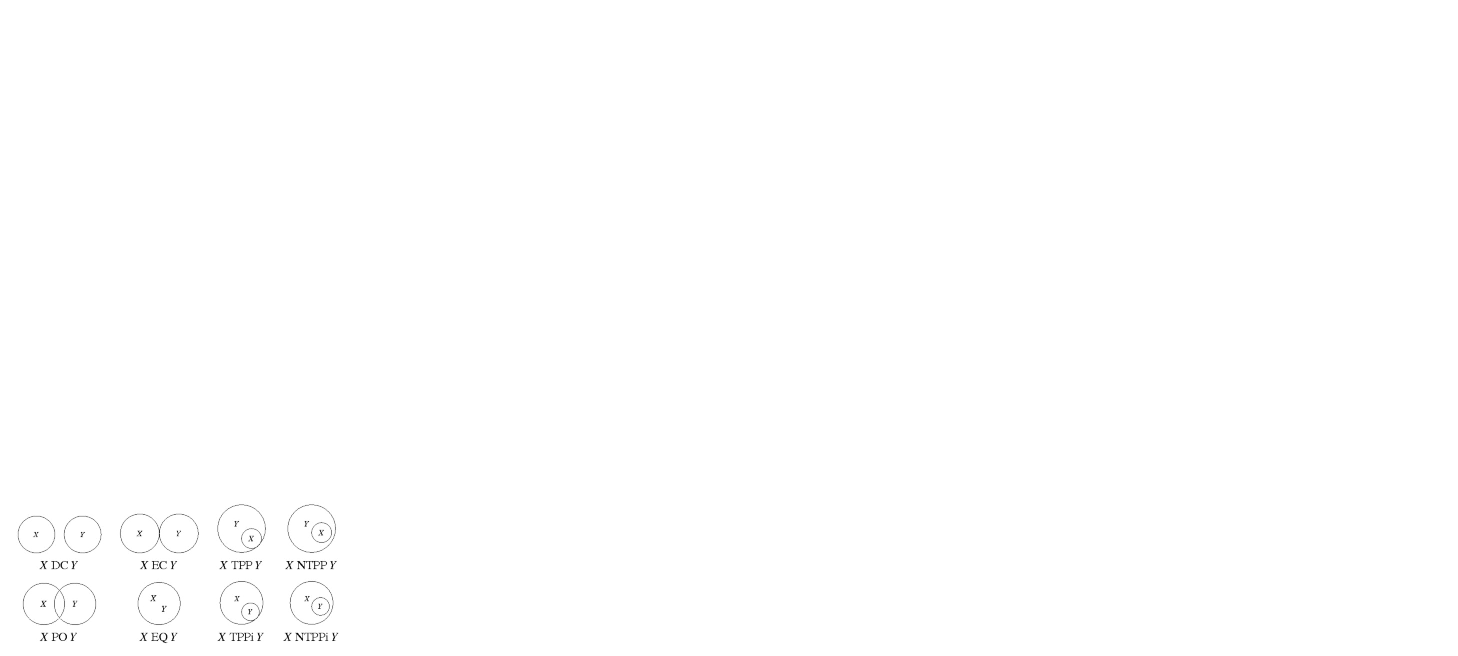
\includegraphics[width=8cm]{RCC8}
\caption{Relations in the Region Connection Calculus}
\label{fig:RCC8}
\end{figure}
%----------------------------------------

We can compose these relations using logical operators. For example,
For example $PP = TPP \cup NTPP$.  For qualitative reasoning about the
relations between regions, there is a \emph{composition
  table}\cite{Cohn1997}. Given the relation $R_1$ between $x$ and $y$
and the relation $R_2$ between $y$ and $z$, the composition table
allows us to determine $R_3$, the relation between $x$ and $z$. We
write this as $R_1 \cdot R_2 \imp R_3$, which translates to $xR_1y,
yR_2z \imp xR_3z$. For example $NTPP \cdot NTPP \imp NTPP$ (i.e
transitivity of non-tangential proper part).

RCC-8 is commonly used in geographical information systems. It could
also be of use in reasoning about biological or biochemical entities
in any number of dimensions. One consideration is that RCC-8 operates
over continuous regions, rather than discrete units, such as
nucleotides.

% ~~~~~~~~~~~~~~~~~~~~~~~~~~~~~~~~~~~~~~~~
\subsection{Allen's Interval Algebra}
% ~~~~~~~~~~~~~~~~~~~~~~~~~~~~~~~~~~~~~~~~

Allen's Interval Algebra (AIA)\cite{allen_maintaining_1983} defines
possible relations between time intervals, and operations on these
intervals, that can be used as a basis for qualitative reasoning about
temporal descriptions of events.

The AIA defines 13 pairwise disjoint base relations that capture all
possible relations between two intervals. The 13 relations consist of
6 asymmetric relations: \emph{precedes (p), meets (m), overlaps (o),
  finishes (f), contains (di), starts (s)}, their inverses:
\emph{precededBy (pi), metBy (mi), overlappedBy (oi), finishedBy (fi),
  containedBy\footnote{sometimes called ``during''} (c), startedBy
  (si)}, and the symmetric \emph{equals (e)} relation.

Composing relations together gives a total possible 8192
relations. The composition operators are intersection ($\cap$), union
($\cup$) and complementation ($\n$). For example, the union $p \cup
pi$ holds whenever two time intervals have no time point in common.

Satisfiability is NP-Complete with AIA i.e. given a collection of
intervals and the relations that hold between them we cannot in
general compute if there are time values for which the relations are
true. However, there are tractable sub-algebras for which efficient
decision procedures exist\cite{Krokhin03reasoningabout}.

Whilst the AIA is generally described as consisting of temporal
intervals, it can be applied to any kind of interval, including
genomic intervals. One consideration is that like RCC-8, the AIA
assumes continuous intervals, rather than discrete intervals.

%Note that the Allen overlaps (o) relation does not correspond to what
%one might understand intuitively by ``overlaps''. The intuitive sense,
%that is, having a sub-interval in common is captured by $o \cup f \cup
%d \cup s \cup e \cup oi \cup fi \cup di \cup si$.

% ~~~~~~~~~~~~~~~~~~~~~~~~~~~~~~~~~~~~~~~~
\subsection{Outline}
% ~~~~~~~~~~~~~~~~~~~~~~~~~~~~~~~~~~~~~~~~

TODO

% ========================================
\section{Results}
% ========================================

% ~~~~~~~~~~~~~~~~~~~~~~~~~~~~~~~~~~~~~~~~
\subsection{An Algebra of Genomic Intervals}
% ~~~~~~~~~~~~~~~~~~~~~~~~~~~~~~~~~~~~~~~~

We base our Genomic Interval Algebra (GIA) on the Allen Interval
Algebra (AIA), and extend it with additional relations requires for
reasoning about DNA sequences. AIA is more suited than RCC-8 for a
basis as genome intervals, like tenporal intervals are directional. We
change some of the terminology of Allen (e.g. using ``upstream'' and
``downstream'' instead of ``precedes'' and ``precededBy''), and take
some terms from RCC-8 (e.g. ``adjacent''), but use Allen-based
definitions.

When considering the biological meaning of these relations, it is
important to stress that they hold between {\em sequences} or
\emph{sequence intervals} (i.e. primary structures) and not the
molecules that are the bearers of those sequences. For example, an RNA
molecule or intron may exhibit connectedness/adjacency between bases
at the secondary structure level. Similarly, a transcription factor
protein may exhibit binding between its amino acid chain and the DNA
sequence upstream of a gene. We consider both these cases to be
non-adjacent and disconnected at the sequence level.

The core of the GIA consists of 16 basic relations $R^{16}$ that can hold
between any two intervals on the same strand of a sequence, defined in
terms of Allen relations. Whilst the IAI treats intervals as
primitives, we also provide definitions in terms of junctions (the
equivalent being time-points in a temporal calculus), yielding a
junction calculus.  We then extend the core set of relations to
account for strandedness, deriving an additional 32 relations.

%----------------------------------------
\begin{figure}
\center
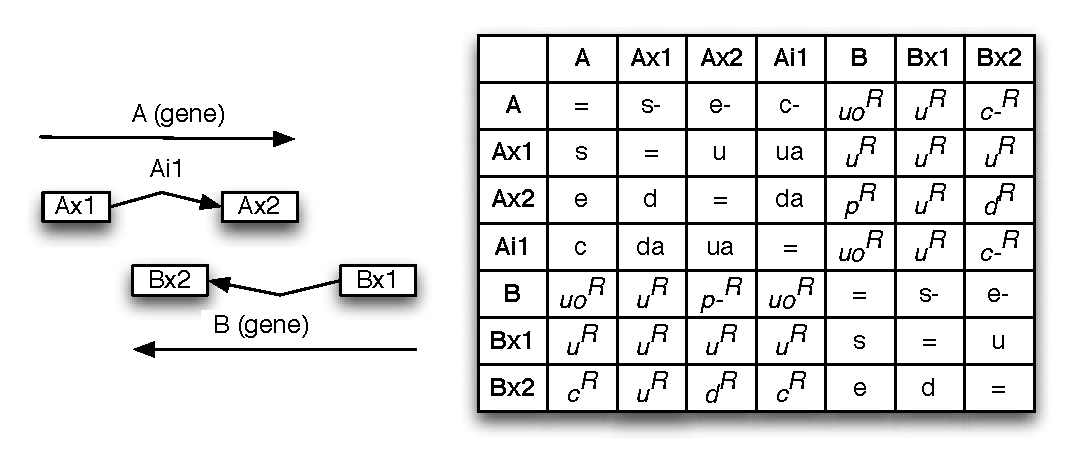
\includegraphics[height=5cm]{relations-examples}
\caption{Example of genomic sequence interval relations: two
  interleaved genes A and B on opposite strands. The lookup table
  shows the mnemonics for the relations between any two feature
  intervals. To determine the relation xRy, look up (row:x
  column:y). For example the first exon of A (Ax1) is upstream of the
  reverse-complement projection of all the exons of B.}
\label{fig:relations-examples}
\end{figure}
%----------------------------------------

Figure \ref{fig:relations-examples} illustrates these relations with a
simplified example.

% ~~~~~~~~~~~~~~~~~~~~~~~~~~~~~~~~~~~~~~~~
\subsubsection{Basic single-strand relations}
% ~~~~~~~~~~~~~~~~~~~~~~~~~~~~~~~~~~~~~~~~

We have declared 16 interval relations that can hold between two
intervals on the same strand of a sequence. These are shown in table
\ref{tab:relations}.

\begin{table}
\begin{tabular}{ | p{5mm} | p{3cm} | p{3cm} | p{3cm} | }
\hline
S & Relation  & Allen Definition  & Inverse \\
\hline
$u$ & \upstreamOf {} & $p$ 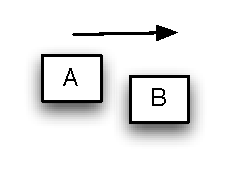
\includegraphics[height=1cm]{u}  & $d$ \small{\downstreamOf} \\
\hline
$a$ & \adjacentTo & $m \cup mi$ & $a$  [symmetric] \\
\hline
$ua$ & \small{\upstreamAdjacentTo} {} & $m$ 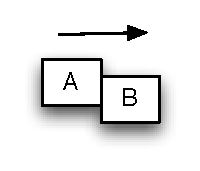
\includegraphics[height=1cm]{ua}   & $da$ \small{\downstreamAdjacentTo} \\
\hline
$uo$ & \small{\upstreamOverlaps} {} & $o$ 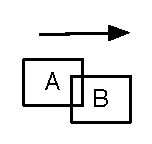
\includegraphics[height=1cm]{uo} & $do$ \small{\downstreamOverlaps} \\
\hline
$o$ & \overlaps & $o \cup f \cup c \cup s \cup e \cup si \cup ci \cup fi \cup oi$  & $o$ [symmetric] \\
\hline
$!o$ & \disconnectedFrom & $p \cup m \cup mi \cup pi$  & $!o$ [symmetric] \\
\hline
$=$ & \coextensiveWith {} &  $e$  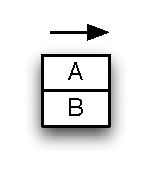
\includegraphics[height=1cm]{eq}  & $=$ [symmetric] \\
\hline
$s$ & \starts {} & $s$ 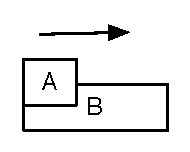
\includegraphics[height=1cm]{s} &  $s-$ \small{\startedBy} \\
\hline
$f$ & \finishes {} & $f$ 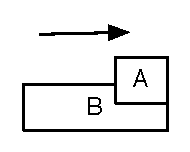
\includegraphics[height=1cm]{f} &  $f-$ \small{\finishedBy} \\
\hline
$c$ & \containedBy {} & $c$ 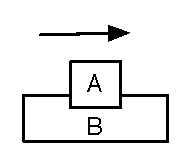
\includegraphics[height=1.2cm]{p} &  $c-$ \small{\contains} \\
\hline
\end{tabular}
\caption{16 Core Relations in the Genome Interval Algebra. Glyphs depict
  the relation holding between A and B, with the strand indicated by an arrow.
  This table provides definitions based on Allen relations. We provide both human-friendly names (e.g. \upstreamOf) and mnemonics (e.g. $u$) }
\label{tab:relations}
\end{table}

Some relations are defined in terms of other relations using
relation-intersection and relation-union operators. These are defined as follows:

intersection: $ x (R \cap S) y \dimp x R y \con x S y$

union: $ x (R \cup S) y \dimp x R y \dis x S y$

complement: $ x (!R) y \dimp \n [ x R y ]$

Note that we do not take the same set of primitives as Allen; we
choose our set based on utility within genome databases and in the
SO. This means that there is not an isomorphic correspondence between
the GIA and Allen. We provide Allen-based definitions using relation
intersection and and union. Unlike Allen, our set is not pairwise
disjoint. For example, $\adjacentTo = \upstreamAdjacentTo \cap
\downstreamAdjacentTo$. We also make different terminological choices
from the IAI. For example, we use \overlaps\ in a more general sense,
in accord with how this term is typically use in bioinformatics, and
how it is defined in the Relation Ontology.

% ~~~~~~~~~~~~~~~~~~~~~~~~~~~~~~~~~~~~~~~~
\subsubsection{Junction-based definitions}
% ~~~~~~~~~~~~~~~~~~~~~~~~~~~~~~~~~~~~~~~~

We also provide definitions for all interval relations in terms of
point-positions or junctions. We define a \emph{proper junction} as a
discrete point connecting two nucleotide bases. Junctions are the union
of proper junctions and the outermost boundary points of a sequence
(this inclusive definition of junction simplifies the axioms).

We define two functions $\alpha$ and $\omega$ each of which maps an
interval to a point (junction), correspoding to the start and end of
the interval. We introduce a relation \succ\ which holds between two
junctions separated by a base, such that the first is at the 5' end
and the second is at the 3' end. We overload the symbol $<$ as the
transitive version of this relation: $x<y \dimp \succ(x,y) \dis \E z:
(\succ(x,z),z<y$. We use $>$ as the inverse of this relation and
define $<=$ as the union of $<$ and $=$ and $>=$ as the union of $>$
and $=$. In the sequence ontology we give these full names such as
\upstreamOfJ.

For any interval, the start is before the end. Formally:

$$
\A x : Interval(x) \imp \alpha(x) < \omega(x)
%\A x : Interval(x) \imp \alpha(x) < \omega(x) \dis \alpha(x) = \omega(x)
$$

Both $<$ and $>$ are irreflexive, and for any non-circular genome they
are anti-symmetric i.e. $\n \E x,y : x<y, y<x$.

%(we allow for zero-length intervals here, i.e. junctions, see below)

%Note that if $<$ and $>$ here do not operate on numbers. If we want a
%numerical interpretation then $\alpha$ and $\omega$ should map to a
%pair (seq,position), with $<$ and $>$ having normal semantics over
%position but always returning false when non-identical sequences.

%Alternatively we could have made the functions map to integers, and
%write out the rules more explicitly; e.g. $ \alpha(x) <= \omega(y)
%\wedge sameSeqAndStrand(x,y)$ for \upstreamOf. This is more akin to
%standard database representations.

\begin{table}
\begin{tabular}{ | p{5mm} | p{5cm} | p{8cm} | }
\hline
S & Relation  & Junction Definition \\
\hline
$u$ & \upstreamOf {} 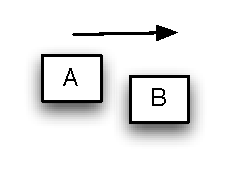
\includegraphics[height=1cm]{u}  & $\omega(x) <= \alpha(y)$ \\
\hline
$ua$ & \upstreamAdjacentTo  & $\omega(x)=\alpha(y)$ \\
\hline
$a$ & \adjacentTo  & $\alpha(x) = \omega(y)  \vee  \omega(x)=\alpha(y)$ {} (derived from: $ua \cup da$) \\
\hline
$uo$ & \small{\upstreamOverlaps} {} 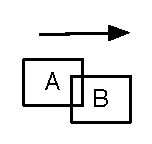
\includegraphics[height=1cm]{uo}  & $\alpha(x) < \alpha(y) \con \omega(x) < \omega(y) \con \alpha(y) < \omega(x)$ \\
\hline
$o$ & \small{\overlaps}  & $\omega(x) > \alpha(y) \con \alpha(x) < \omega(y)$  \\
\hline
$!o$ & \small{\disconnectedFrom}  & $\omega(x) <= \alpha(y) \vee \alpha(x) >= \omega(y)$ {} (derived from: $\n o$)\\
\hline
$s$ & \starts {} 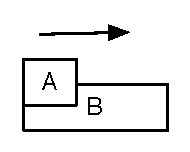
\includegraphics[height=1cm]{s}  & $\alpha(x) = \alpha(y) \con \omega(x) < \omega(y)$ \\
\hline
$f$ & \finishes {} 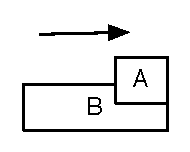
\includegraphics[height=1cm]{f}  & $\alpha(x) > \alpha(y) \con \omega(x) = \omega(y)$ \\
\hline
$c$ & \containedBy {} 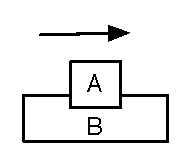
\includegraphics[height=1.2cm]{p} & $\alpha(x) >  \alpha(y) \con \omega(x) < \omega(y)$ \\
\hline
$=$ & \coextensiveWith {} 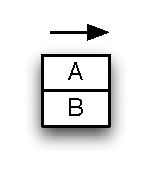
\includegraphics[height=1cm]{eq}  &  $\alpha(x)=\alpha(y) \con \omega(x)=\omega(y)$ \\
\hline
\end{tabular}
\caption{Junction-based definitions. Definitions are not shown for inverses, which can be trivially obtained by reversing $x$ and $y$.}
\label{tab:junction-defs}
\end{table}

Table \ref{tab:junction-defs} gives the definition of interval relations
in terms of junctions.

We can eliminate the function terms from the definitions by
translating to composition rules such that for example:

$$
\omega(x) <= \alpha(y) \dimp \upstreamOf(x, y)
$$

Is translated to:

$$
\hasOmega(x,x_s),\beforeOrOn(x_s, y_e), \alphaOf(y_e,y) \dimp \upstreamOf(x,y)
$$

We can eliminate the variables using an equivalence assertion and a
relation chain:

$$
\hasOmega \cdot \beforeOrOn \cdot \alphaOf \dimp \upstreamOf(x,y)
$$

Here \hasAlpha\ and \hasOmega\ are a functional relations between a region
and a junction, with inverses \alphaOf\ and \omegaOf.

%[CHECK: no longer closed so is this still an algebra?]. 
These additional relations give us an algebra over junctions and
relations which we call $GIA^J$, which can be used with qualitative
reasoning systems. Note the correspondence of \succ\ to the function
$+1$ and between $<$ and $>$ and their arithmetic counterparts -- the
correspondence allows the use of either artihmetic operations or
qualitative reasoning.

% ~~~~~~~~~~~~~~~~~~~~~~~~~~~~~~~~~~~~~~~~
\subsubsection{Derived Reverse-Complement Relations}
% ~~~~~~~~~~~~~~~~~~~~~~~~~~~~~~~~~~~~~~~~

The major difference between temporal and genomic intervals is that
DNA is stranded. The GIA must therefore be an \emph{extension} of the
AIA to fully account for strandedness.

We treat each strand of a double-stranded DNA molecule as bearing two
distinct sequence intervals $s^+$ and $s^-$, related by the \rc\
relation. Each junction $j_a^+$ on $s^+$ has a unique single cognate
junction $j_a^-$ on $s^-$ related via \rc\ such that upstream and
downstream are reversed:

$$\succ(j_a^+,j_b^+), \rc(j_a^+,j_a^-), \rc(j_b^+,j_b^-) \dimp \succ(j_b^-,j_a^-)$$

Further axioms can be added to state the relationship between base
types on opposing strands (not shown here).

For any genome interval relation in $r \in R^{16}$, we can define a
reverse-complement cognate, $r^{R}$. We obtain definitions for these
automatically using the formula:

$$r^{R}(x,y) = r(x,\rc(y))$$

In table \ref{tab:RCrelations} we show only one \rc\ relation,
\upstreamOverlapsRC. This is equivalent to \upstreamOverlaps\ with
\rc\ applied to the second argument. Note that unlike
\upstreamOverlaps, this is a symmetric relation. Conversely,
\containedByRC\ (not shown), \textbf{is} the inverse of \containsRC. See
figure \ref{fig:relations-examples} for an illustration of why this is
the case.

For any $r \in R^{16}$, we can further define a relation $r^{U} = r
\cup r^{R}$. Table \ref{tab:RCrelations} illustrates this with
$\upstreamOverlapsRC \cup \upstreamOverlaps$ which we call this
\upstreamOverlapsU.  These union relations correspond to
common use cases (e.g. Region-of-Interest queries in Genome
Browsers\cite{Stein2002}\cite{skinner2009jbrowse}\cite{Lewis2002}), so
we should have intuitive names for them. However, from the point of
view of axiomatisation, it is simpler to treat these as derived rather
than basic relations.

Thus we have 16 relations in the core set (including inverse relations
for non-symmetric relations).  We declare relations for this core set,
plus their $\rc$ equivalents, plus the union set. This gives us 48
relations in total. This may seem excessive but as we will see we will
need most for our use cases.

\begin{table}
\begin{tabular}{ | p{3cm} | p{4cm} | p{4cm} | }
\hline
Relation  & Definition & Inverse \\
\hline
$uo$ \small{\upstreamOverlaps} {} 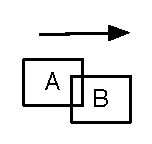
\includegraphics[height=1cm]{uo} & $\alpha(x)<\alpha(y) \con$ $\omega(x)<\omega(y) \con$ $\alpha(y)<\omega(x)$ & $do$ [\downstreamOverlaps] \\
\hline
$uo^R$ \upstreamOverlapsRC  {} 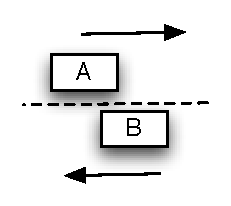
\includegraphics[height=1.2cm]{uoR} & $\alpha(x)<\alpha(\rc(y)) \con$ $\omega(x)<\omega(\rc(y)) \con$ $\alpha(\rc(y))<\omega(x)$ & [symmetric] \\
\hline
$uo^*$ \upstreamOverlapsU   & $uo^R \cup uo$ & $uo^R \cup do$ \\
\hline
\end{tabular}
\caption{Example of Reverse Complementation cognate relations for the \upstreamOverlaps\ relation. Note the interaction between RC and inverse relations: in particular the inverse of $uo^R$ does not correspond to a single named relation. }
\label{tab:RCrelations}
\end{table}

% ~~~~~~~~~~~~~~~~~~~~~~~~~~~~~~~~~~~~~~~~
\subsubsection{Operations over collections of intervals}
% ~~~~~~~~~~~~~~~~~~~~~~~~~~~~~~~~~~~~~~~~

Many genomic features correspond to \emph{collection} of intervals on
a sequence - for example, the coding part of a multi-exon gene.
Neither RCC-8 not AIA dictate operations over collections of regions
or intervals. We propose a simple extension in GIA for dealing with
such collections.

We overload the relations that are used for single intervals, but
provide distinct definitions. We also define new relations that
are only applicable to collections. For example, in figure
\ref{fig:relations-examples} genes A and B stand in an $o^{R}$
(overlaps) relation, even though their respective exons share no
bases. However, we can introduce a new relation \interleavesR, defined
such that the exons in gene A interleave (on the opposite strand) the
exons in gene B. (note that it is important that we distinguish
between the sets of exons interleaving and the genes overlapping).

We present here a subset of the full set of relations, which have yet
to be finalized. We treat each collection as a set of intervals.

Overlaps must hold for some pair of elements from each pair:

$$\overlaps(X,Y) \dimp \E x,y : x \in X \con y \in Y \con \overlaps(x,y) $$

Adjacency must hold of any one pair, and in addition there should be no overlap:

$$\adjacentTo(X,Y) \dimp \E x,y : x \in X \con y \in Y \con \adjacentTo(x, y) \con \n \overlaps(X,Y)$$

Upstream must hold for all elements:

$$\upstreamOf(X,Y) \dimp \A x,y : (x \in X \con y \in Y \imp \upstreamOf(x,y) )$$

Interleaves is more complex:

\begin{equation*}\begin{split}
\interleaves^{R}(X,Y) & \dimp \E (x_1 \in ,x_2 \in X,y_1 \in Y,y_2 \in Y) : \\
& \upstreamOfRC(x_1,  y_2) \con \\
& \downstreamOfRC(x_1, y_1) \con \\
& \downstreamOfRC( x_2, y_2) \con \\
& \n \overlapsRC(X, Y)\\
\end{split}\end{equation*}



% DISCUSSION:
%Another application of these collection-based relations is for
%reasoning over the projections of RNA secondary structures on genomic
%sequence.

% ~~~~~~~~~~~~~~~~~~~~~~~~~~~~~~~~~~~~~~~~
\subsubsection{Composition table}
% ~~~~~~~~~~~~~~~~~~~~~~~~~~~~~~~~~~~~~~~~

The full composition table for GIA(J) is too large to show but is
available as part of the Genome Intervals relations file. Some
examples include:

Transitivity of\upstreamOf:

$$
\upstreamOf \cdot \upstreamOf \imp \upstreamOf
$$

\starts\ and \finishes\ compose to make (non-tangential) containment:

$$
\starts \cdot \finishes \imp \containedBy
$$

The RC upstream of relation is transitive over downstream of (consider
Ax1 u Bx2 d Bx1 in figure \ref{fig:relations-examples}):

$$
\upstreamOfRC \cdot \downstreamOf \imp \upstreamOfRC
$$

The full composition table was derived by an automated theorem prover (see methods).

%[Include proofs from Prover9?]

% ~~~~~~~~~~~~~~~~~~~~~~~~~~~~~~~~~~~~~~~~
\subsection{Applications}
% ~~~~~~~~~~~~~~~~~~~~~~~~~~~~~~~~~~~~~~~~

% ~~~~~~~~~~~~~~~~~~~~~~~~~~~~~~~~~~~~~~~~
\subsubsection{Numeric Genome Interval Queries}
% ~~~~~~~~~~~~~~~~~~~~~~~~~~~~~~~~~~~~~~~~

Given a genomic dataset consisting of features with intervals with
specified start and end positions....

% ~~~~~~~~~~~~~~~~~~~~~~~~~~~~~~~~~~~~~~~~
\subsubsection{Relative Genome Interval Queries}
% ~~~~~~~~~~~~~~~~~~~~~~~~~~~~~~~~~~~~~~~~

% ~~~~~~~~~~~~~~~~~~~~~~~~~~~~~~~~~~~~~~~~
\subsubsection{Genome Dataset Validation}
% ~~~~~~~~~~~~~~~~~~~~~~~~~~~~~~~~~~~~~~~~

% ~~~~~~~~~~~~~~~~~~~~~~~~~~~~~~~~~~~~~~~~
\subsubsection{Class-level Reasoning}
% ~~~~~~~~~~~~~~~~~~~~~~~~~~~~~~~~~~~~~~~~


% ~~~~~~~~~~~~~~~~~~~~~~~~~~~~~~~~~~~~~~~~
\subsection{Extending the Sequence Ontology}
% ~~~~~~~~~~~~~~~~~~~~~~~~~~~~~~~~~~~~~~~~

We can use the genome interval relations above to extend the SO,
adding new logical definitions and constraint axioms -- we call the
resulting artefact \SOGI. These logical definitions can be used for
both reasoning within the ontology, and to infer the presence of
unstated genomic features in genome databases. The constraint axioms
can be used to detect inconsistencies within the ontology, and to
provide constraints for genome databases.

% ~~~~~~~~~~~~~~~~~~~~~~~~~~~~~~~~~~~~~~~~
\subsubsection{Logical Definitions}
% ~~~~~~~~~~~~~~~~~~~~~~~~~~~~~~~~~~~~~~~~

Logical definitions provide necessary and sufficient conditions in
computable form. We have created 140 new definitions for existing SO
types based on the GIA relations. Table \ref{tab:definitions} shows a
subset of these. SO uses the type-level version of these relations

\begin{longtable}{ | c | c | p{5cm} | }
\hline
Type  & Genus & Differentia \\
\hline
\fivePrimeCodingExon  & \codingExon  & \rel{\overlaps\ \startCodon} \\
\hline
\fivePrimeIntron  & \intron  & \rel{\containedBy\ \fivePrimeUTR} \\
\hline
\UTRIntron  & \intron  & \rel{\overlaps\ \UTR} \\
\hline
\twintron  & \intron  & \rel{\containedBy\ \intron} \\
\hline
\startCodon  & \codon  & \rel{\starts\ \CDS} \\
\hline
\stopCodon  & \codon  & \rel{\finishes\ \CDS} \\
\hline
%\intergenicRegion & \region & $\disconnectedFrom\ \gene$ $\adjacentTo(2) \gene$ \\
\intergenicRegion & \region & \rel{\disconnectedFrom\ \gene} \rel{\upstreamAdjacentTo \gene} \rel{\downstreamAdjacentTo \gene} \\
\hline
\noncodingExon & \exon & \rel{\disconnectedFrom\ \CDS} \\
\hline
\intron & \region & \rel{\containedBy\ \transcript} \rel{\upstreamAdjacentTo\ \exon} \rel{\downstreamAdjacentTo\ \exon} \rel{\disconnectedFrom\ \exon} \\
\hline
\interiorIntron & \intron & \rel{\containedBy\ \CDS} \\
\hline
\fivePrimeUTR  & \mRNARegion  & \rel{\upstreamAdjacentTo\ \CDS} \rel{\starts\ \mRNA} \\
\hline
\threePrimeUTR  & \mRNARegion  & \rel{\downstreamAdjacentTo \CDS} \rel{\finishes \mRNA} \\
\hline
\interiorUTR  & \mRNARegion  & \rel{\downstreamAdjacentTo\ \CDS} \rel{\upstreamAdjacentTo\ \CDS} \\
\hline
\interiorExon  & \exon  & \rel{\adjacentTo\ \fivePrimeSpliceSite} \rel{\adjacentTo\ \threePrimeSpliceSite} \rel{\disconnectedFrom\ \spliceSite} \\
\hline
\caption{Examples of logical definitions of SO terms using GI
  relations. Relation quantifiers are taken to be All-Some unless otherwise
  noted. The semantics of a genus differentia definition (T,G,D) are
  such that $T(x) \dimp G(x) \con \A (R,Y) \in D : \E y : xRy$}
\label{tab:definitions}
\end{longtable}

% move this later?

Because the definitions are both necessary and sufficient, they can be
used to construct queries on genome databases. For example, to find 5'
coding exons, make a conjunctive query for coding exons that overlap
start codons. $\overlaps $ can be translated to a genome coordinate
query. The query may need further expansion of start codon or coding
exon is not materialized in the database.

% ~~~~~~~~~~~~~~~~~~~~~~~~~~~~~~~~~~~~~~~~
\subsubsection{Relationship and Constraint Axioms}
% ~~~~~~~~~~~~~~~~~~~~~~~~~~~~~~~~~~~~~~~~

SO already has relationships between types specified in the ontology:
for example, \rel{\TSS\ \partOfT\ \transcript}, which states that if
$x$ is an instance of a \TSS\ then there must be some \transcript\ $y$
such that $\partOf(x,y)$.

Using the GIA relations we can add new relationships to SO, or refine
existing relationships that may have unclear semantics. Table
\ref{tab:constraints} shows a sample of these. Note that we exclude
the relationships which are trivially obtained from the definitions in
table \ref{tab:definitions}.

\begin{longtable}{ | c | c | }
\hline
Type  & Relationship \\
\hline
\TSS  & \rel{\upstreamOf\ \primaryTranscript}  \\
\hline
\polyAsequence  & \rel{\downstreamAdjacentTo\ \mRNA} \\
\hline
\polyAsite  & \rel{\omegaOf\ \mRNA} \\
\hline
\caption{Proposed new relationship axioms for SO using genome interval
  relations. These are type-level relationships that can be translated
  to instance level relationships such that for example $\TSS(x) \imp
  \E y, \primaryTranscript(y), \upstreamOf(y)$}
\label{tab:constraints}
\end{longtable}

%Given the above we may want to say $\TSS
%\upstreamOf proj(\primaryTranscript, \genome)$. Here we abbreviate
%this as $\TSS \upstreamOf \genome(\primaryTranscript)$.

We can use these type-level relationships as constraints on a genome
database. We must do this carefully, bearing in mind the fact that
these axioms make an open-world assumption: just because an instance
in reality is entailed to exist, it does not follow that this musy be
explicitly represented in the genome database.

Note that many of the relationships in table \ref{tab:constraints} are
in fact \emph{underconstrained} as constraints. For example, take
\rel{\TSS\ \upstreamOf\ \primaryTranscript}. This is in fact an extremely
weak axiom - it states that every \TSS\ is upstream of \emph{some}
\primaryTranscript\ - the \TSS\ and \transcript\ do not have to be
otherwise related. This will be trivially true: a \TSS\ located at the
end of a chromosome sequence will be upstream of \emph{all} the other
genes on the same strand.

In fact we want to say that every \TSS\ lies upstream \emph{of the
  same transcript that it regulates}. The current version of SO uses
a \partOfT relation between the \TSS\ and the \primaryTranscript\ to
indicate that every \TSS\ is functionally coupled to a
\primaryTranscript. We can write a fully constrained axiom:

$$
\partOf(x,y) \con \TSS(x) \con \transcript(y) \imp \upstreamOf(x,y)
$$

We can use this axioms to check instance-level data, as found in
genome databases and data files.

%Note that these logical constraints go beyond what can be done with
%normal ontology graph edges. We include Nnn axioms of this variety in
%the extended SO, encoded as \emph{formulae} in the OBO format.

%TODO: Codon example

% Bidirectional promoter

% ~~~~~~~~~~~~~~~~~~~~~~~~~~~~~~~~~~~~~~~~
\subsection{Reasoning  over genome intervals}
% ~~~~~~~~~~~~~~~~~~~~~~~~~~~~~~~~~~~~~~~~

We can use \SOGI (the combination of the SO extended with GIA
relations) to perform reasoning tasks. These tasks can be broken down
according to whether we are performing \emph{validation} of axioms or
\emph{inference} of unstated axioms. We can further break this down
according to whether we are performing reasoning over just \SOGI, or
the combination of \SOGI and some genomic instance data.

We can use a number of different systems for reasoning. Relational
databases are generally considered to be the least expressive (meaning
that we cannot translate some axioms to the relational model), but are
also considered to scale to large genome-sized datasets. At the other
extreme are first-order logic theorem provers, which allow for high
expressivity, but do not scale well. In between there are a number of
different systems that can be roughly divided into partially
overlapping rule-based and description-logic (DL) approaches.

Rule based approaches extend the expressivity of the relational model
with arbitrary recursive rules; the OBO-Edit reasoner is an example of
a rule-based system. More expressive systems include disjunctive
datalog engines such as DLV. OWL-DL (Web Ontology Language Description
Logic) was designed to maximine expressivity and decidability, and
there are a variety of OWL-DL reasoners.

The set of relations consisting of the core 16 basic GIA relations do
not correspond to any of the tractable sub-algebras of the Allen
Algebra (for example, the \adjacentTo\ relation, defined in terms of
Allen as $m \cup mi$ appears in none of the tractable
subsets). However, this is not a major concern for the majority of
genome databases in which interval junctions can always be assigned to
discrete ordered bases.

We present first examples of reasoning using \SOGI, and then examples
of reasoning using a combination of \SOGI and genome databases.

\subsubsection{Reasoning over the ontology}

Given an ontology consisting of a set of \emph{asserted}
relationships, a reasoner can infer the \emph{entailed}
relationships. The full set of entailed relationships for a relation
$R$ is called the \emph{deductive closure} of $R$.

Computing entailed relationships is useful for ontology maintenance -
the \isA\ hierarchy for 200 of the terms in SO is maintained
automatically be the OBO-Edit reasoner, using the existing
genus-differentia definitions.

Computing the deductive closure of all ontology relations is also
useful for improving genome database queries.

Given that the SO is by itself several orders of magnitude smaller
than a typical genome database, we can afford to use a system with
higher expressivity to do the reasoning. We have used both OBO and
OWL-DL reasoners to compute entailed relationships in \SOGI, and both
give the same results.

In theory an OWL-DL reasoner can compute relationships that are
difficult to compute using a rule-based approach. For example,
inferring that every codon overlaps a CDS, based on the five axioms:
(a) a codon is either a start or stop codon (b) start codons start a
CDS, and (c) start implies overlaps (d) stop codons stop a CDS, and
(e) stop implies overlap. Currently the OBO-Edit reasoner does not
make use of class unions. In this particular case it doesn't matter,
as the relationship was already asserted at the codon level.

%The OE reasoner can make use of relation intersections (unlike OWL
%reasoners), but no useful inferences were found using these.

Figure \ref{fig:qualitative-reasoning} shows examples of entailed
relationships. We can ask \emph{how are the type 5'UTR and start codon
  related?} and get the answer \upstreamAdjacentTo, even though this
fact is not explicitly stated in the ontology.

%----------------------------------------
\begin{figure}
\center
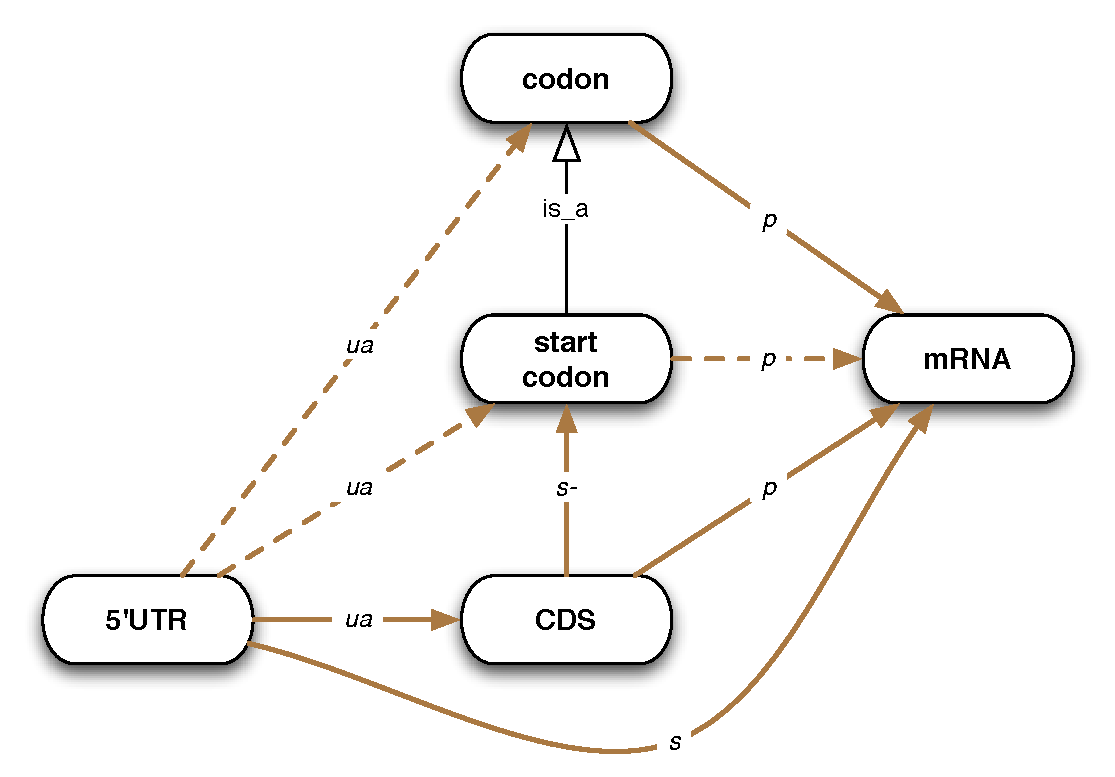
\includegraphics[height=5cm]{qualitative-reasoning}
\caption{Reasoning over ontologies: this example illustrates the
  deductive closure involving a few SO types, and makes use of the
  relation composition axiom $\upstreamAdjacentTo \cdot \startedBy
  \imp \upstreamAdjacentTo$ to infer that every \rel{\fivePrimeUTR\
    \upstreamAdjacentTo\ \startCodon} (inferred relationships are
  shown with dashed lines). Not all inferences are shown. This is an
  example of qualitative/symbolic reasoning - we can make inferences
  even without arithmetic, using the GIA}
\label{fig:qualitative-reasoning}
\end{figure}
%----------------------------------------


%The OWL reasoners were able to infer subsumption relations where
%cardinality is involved - e.g. \emph{dicistronic transcript \isA
%  polycistronic transcript}; the OE reasoner needs extended to do
%this.

%Both reasoners were unable to make inferences where n-ary relations
%are involved.

The other application of reasoning over ontologies is to find
inconsistencies or unsatisfiable classes.  Using both OBO-Edit and
OWL-DL reasoners, we could find no inconsistencies between axioms
within the extended SO. This is not surprising as the SO is carefully
scrutinized by its editors prior to each release, and automated
procedures are currently in use with the existing axioms. We still
expect that the extended SO presents more precise axioms on which
these reasoners can operate.

An example of a conceivable mistake that can be detected by reasoners
is: (a) \rel{\threePrimeUTR\ \downstreamAdjacentTo\ \CDS} (b)
\rel{\stopCodon\ \isA\ \codon} (c) \rel{\codon\ \containedBy\ \CDS}
(d) \rel{\stopCodon\ \starts\ \threePrimeUTR}. This example is not
entirely artificial: prior to the existence of SO there was
inconsistency amongst the genomics community as to whether the stop
codon should be considered part of the CDS. This inconsistency caused
interoperability problems, which were solved for systems adopting SO.

%[TODO: deliberately put some nonsense in the ontology and detect
%inconsistency]

%However, we did find some inferences that were not flagged as
%inconsistent, that were nevertheless unusual. For example, based on
%the adjacency relation between a \polyAsequence and an \mRNA, [TODO:
%discussion of genome vs transcriptome problem]

\subsubsection{Towards reasoning over genome datasets}

%[TODO: move section on validation from introduction here?]

Whilst making inferences over and checking the validity of ontologies
is undoubtedly useful for ontology manintence, a more relevant use
case for bioinformatics is reasoning over genome datasets, using the
ontology as a computable specification.

The size of genome datasets vary tremendously according to the
organism(s) being studied and the type of questions being asked, but
even the smallest datasets are typically contain orders of magnitude
many more assertions than an ontology such as SO. We would expect that
most current OWL-DL reasoners (which typically reside in-memory) would
not perform well on genome datasets. We would also expect relational
engines to perform better, but to give incomplete results in the
absence of certain kinds of explicitly asserted information. An
interesting middle-ground is that occupied by \emph{deductive
  databases} - these are typically extensions of the relational model
with the addition of recursive rules (Datalog). We were also
interested in the performance and expressivity of hybrid
relational-OWL systems such as OWLGRES.

In order to test these systems, we had to define a number of mappings
and implement a generalized translation system, described in the
methods section. The system takes as input \SOGI (expressed in OBO and
First-Order Logic) and one of more datasets (which can be GFF3 files
or remote Ensembl or Chado databases). The system will then translate
queries or constraints to the underlying reasoning system. This system
is not complete, but it allows us to explore the expressivity and
scalability of the different systems.

% TODO

% ========================================
\section{Discussion}
% ========================================

% ~~~~~~~~~~~~~~~~~~~~~~~~~~~~~~~~~~~~~~~~
\subsection{Enhanced rigor in the Sequence Ontology}
% ~~~~~~~~~~~~~~~~~~~~~~~~~~~~~~~~~~~~~~~~

In describing the GIA and extending SO we came across portions of SO
that were in need of more precise textual definitions. For example,
\intergenicRegion\ was defined as \emph{A region containing or
  overlapping no genes that is bounded on either side by a gene}. In
formalizing the definition for this using the \upstreamAdjacentTo\ and
\downstreamAdjacentTo\ relations to represent \emph{bounded on either
  side} we realized that this definition excluded the two regions on
either end of a chromosome. The textual definition was extended to be
include the disjunctive clause \emph{or bounded by either a gene or
  the end of the chromosome}. Another example was \spliceSite, which
had a textual definition indicating that it was a junction but a
placement in the \isA hierarchy indication a region. Once the
computable definition was added, the inconsistency could be detected
by a reasoner (although it was in fact detected whilst preparing the
logical definition). This resulted in the definition being clarified
and the addition of a new term \spliceJunction.

% ~~~~~~~~~~~~~~~~~~~~~~~~~~~~~~~~~~~~~~~~
\subsection{Junction-oriented vs Base-oriented}
% ~~~~~~~~~~~~~~~~~~~~~~~~~~~~~~~~~~~~~~~~

Our formulation is a junction or \emph{interbase} one. We could
equally have defined interval relations in terms of the bases
themselves. We consider an interbase system to have a slight advantage
in terms of simplicity of representation of positioning of splice
junctions, insertion regions and so on. However, the two systems would
be equivalent in terms of expressivity, so the choice of one over the
other is arbitrary.

% ~~~~~~~~~~~~~~~~~~~~~~~~~~~~~~~~~~~~~~~~
\subsection{Unresolved Issues}
% ~~~~~~~~~~~~~~~~~~~~~~~~~~~~~~~~~~~~~~~~

\subsubsection{Splicing, transcripts and exon identity}

The examples presented in this paper make a simplifying assumption,
namely that all types in the SO represent features along a DNA
sequence. The relationships and definitions presented here do not
account for the biology of splicing and translation. For example,
exons are non-adjacent on the DNA sequence and on the unspliced RNA
sequence, but become adjacent after splicing. A full treatment will
have to account for this temporal aspect. One approach is to introduce
different types, such as \exon$^{G}$ and \exon$^{T}$ for exons on
genomes and exons on transcripts respectively. Another is to use n-ary
relations such that it is possible to state \rel{\exon\ \adjacentTo\
  \exon\ \on\ \matureTranscript} and \rel{\exon\ \disconnectedFrom\
  \exon\ \on\ \genome}.

\subsubsection{Circular genomes}

The current axiomatization needs to be modified to handle circular
genomes. One approach is to weaken the definition of $<$ such that it
is reflexive on circular genomes. However, this will have some
consequences for the other axioms, which needs to be fully worked
out. For example, every feature would be upstream of every other
feature.

Another solution would be to have some kind of probabilistic metric or
arbitrary cut-off, whereby junctions are no longer considered upstream
if they loop around the circular DNA too far. But this would be
difficult to integrate into these existing axioms.

The most likely approach is to use origin of replication (oriC in
bacteria) as the origin of the sequence.

% ~~~~~~~~~~~~~~~~~~~~~~~~~~~~~~~~~~~~~~~~
\subsection{Reasoning Systems}
% ~~~~~~~~~~~~~~~~~~~~~~~~~~~~~~~~~~~~~~~~

Navigating the landscape of different representational frameworks and
their reasoning systems can be difficult for bioinformaticians without
a background in mathematical logic. What is clear is that there is no
one system that suits all purposes. 

\begin{clist}

\item Full first-order logic and associated theorem provers are useful
  for reasoning over the set of relations and their properties. Whilst
  not a common activity, this can be vital as a first step to building
  an ontology or defining a set of relations (as in this paper)

\item Description-logic level expressivity is useful for reasoning
  over an ontology. This is a vital part of the ontology development
  cycle, but in itself rarely of use to non-ontologists.

\item Relational and datalog level expressivity and associated engines
  are necessary for reasoning and query answering over genome-sized
  datasets.

\end{clist}

Note that contrary to common belief the expressivity of the relational
model is not a strict subset of the expressivity of description
logics: relational systems allow the definition of relations using
boolean operators, and allow the use of arithmetic in expressions -
vital for fast queries over genomes. In contrast DL ontologies such as
OWL-Time\cite{OWLTime} do not include definitions for relations. It is
possible to define these using the Semantic Web Rule Language (SWRL),
but not the DL-safe subset that is supported by most reasoners.

The findings of this paper indicate one good strategy to be to use the
most expressive language possible at the ontology level, and to
translate to a specific language and implementation as needed,
depending on the use case and question-answering capabilities required.

% ========================================
\section{Conclusions}
% ========================================

We have defined a collection of genome interval relations, and used
them to define an extension of the Sequence Ontology (SO). This
extension and these relations will soon become part of the core
SO. The relations help clarify the meaning of terms in the SO to
humans, and can be used by automated reasoning systems to assist with
the construction and quality control of the ontology.

In additions the relations are useful for querying over and checking
the conformance of datasets to constraints in the SO. The relations
help clarify the meaning of certain queries to human beings, such that
a query for ``all exons upstream of gene ABC'' has precise
semantics. The extended SO can be used to enhance database queries
such that implicit features such as introns are found.
We found the most effective system for querying over genome datasets
was a relational database with the help of a query expansion
system. OWL-DL systems do not yet scale over genome sized datasets.

The composition table is useful for making inferences over the
ontology, but for making inferences over data it is simpler to
use arithmetic definitions rather than a composition table. Similar
conclusions have been made about GIS databases and RCC8\cite{Goodwin}.

We believe that as genome datasets grow in size, complexity and
importance the need for formal computable specifications of genomic
data will increase. Specifications such as the one outlined here will
be vital for ensuring the semantic and biological correctness of
important datasets, and for performing advanced queries over these
datasets.

% ========================================
\section{Methods}
% ========================================

\subsection{Defining the Genome Interval Relations}

We used OBO-Edit\cite{Day-Richter2007} to specify the genome interval
relations and to create an extended subset of SO that used these
relations for genus-differentia definitions. This was stored in an OBO
Format 1.3 file.

\subsection{Generation of composition table}

To generate the full composition table, we first translated the genome
interval relations to Prover9 syntax and used the Prover9 tool to
calculate the table by brute force attempts to prove every possible
$R1 \cdot R2 \imp R$ for all values of $R$, $R1$ and $R2$.

\subsection{Reasoning over \SOGI}

For reasoning over \SOGI we used both the OBO-Edit reasoner and Pellet
[TODO: try again with full composition table]. For the latter we used
the standard obo to OWL translation as specified by Horrocks et
al. Neither the OBO-Edit reasoner nor Pellet made use of the full FOL
axioms.

For OWL reasoning over the ontology, we also materialized classes $\E
R D$ for all $R \in R^{16}$ and all $D \in SO$. This was to allow us
to infer type-level relationships by testing the TBox for subsumption.

For reasoning over \SOGI\ in addition to genome datasets we used a
variety of approaches. We defined mappings from both the Ensembl and
Chado relational models to a Datalog model based on Chado. We can then
dynamically rewrite Datalog queries to SQL using a standard
mapping\cite{Draxler1991}. We also translate \SOGI to Datalog.

Constraint axioms in \SOGI can be translated to SQL checks; for example

$$
\partOf(x,y) \con \TSS(x) \con \transcript(y) \imp \upstreamOf(x,y)
$$

Is translated to a Chado query:

\renewcommand{\ttdefault}{txtt}
\begin{scriptsize}
\lstset{language=SQL,
keywordstyle=\color{black}\bfseries\underbar,
stringstyle=\ttfamily, % typewriter type for strings
basicstyle=\ttfamily,
}
\lstset{linewidth=\textwidth}
\lstset{columns=fullflexible, basewidth={0.5em,0.4em}}
\lstset{frame=trBL,frameround=tttt}

\lstinputlisting[caption=Chado SQL Constraint: this query returns a
list of all invalid TSSs. \pr{feature\_upstream\_of} is an intensional
predicate generated automatically from the relation definitions.
,label=lst:chado-tss]{chado-tss.sql}

\end{scriptsize}

TODO: DLV, XSB

%We used the blipkit to extract feature data from
%GFF3/Chado/Ensembl and to write to other languages, including OWL-DL.

%CGL\cite{Yandell2006}

% ~~~~~~~~~~~~~~~~~~~~~~~~~~~~~~~~~~~~~~~~
\subsection{Availability}
% ~~~~~~~~~~~~~~~~~~~~~~~~~~~~~~~~~~~~~~~~

\SOGI can be downloaded from the SO
repository\footnote{http://www.sequenceontology.org/resources/index.html}. The
extension is called working draft.obo, and the relations are defined
in gia.obo. Versions in Common Logic, Prover9 and OWL-DL are also provided\footnote{http://www.fruitfly.org/\~cjm/ro/ro-genome-interval.html}

% ========================================
\section{Acknowledgements}
% ========================================



% ========================================
\section{References}
% ========================================

\bibliography{genome-intervals}

% this one produces numeric entries in the order they appear BUT not URLs
%\bibliographystyle{unsrt}

% this one does URLs in correct order, but they are not numbered..
\bibliographystyle{unsrtnat}

\end{document}


